% Quality and local-support metrics for the H2 study (Beamer).
% Overleaf: New Project -> Upload Project (this folder), compiler pdfLaTeX.
\documentclass[aspectratio=169,11pt]{beamer}
\usepackage[T1]{fontenc}
\usepackage{amsmath,amssymb,mathtools,bm,booktabs,tabularx,array,graphicx}
\graphicspath{{figures/}}
\usetheme{default}
\setbeamertemplate{navigation symbols}{}
\setbeamertemplate{footline}{\hfill\scriptsize\color{gray}\insertframenumber/\inserttotalframenumber\hspace{1em}\vspace{0.6em}}
\definecolor{acc}{HTML}{1F4E79}
\setbeamercolor{frametitle}{fg=acc}
\setbeamercolor{structure}{fg=acc}
\setbeamercolor{block title}{bg=acc!15,fg=acc}
\setbeamercolor{block body}{bg=acc!4}
\setbeamerfont{frametitle}{series=\bfseries}
\setbeamertemplate{blocks}[rounded]
\newcolumntype{Y}{>{\raggedright\arraybackslash}X}
\DeclareMathOperator{\pct}{pct}
\DeclareMathOperator{\median}{median}
\DeclareMathOperator{\tr}{tr}
\DeclareMathOperator{\sd}{sd}
\newcommand{\R}{\mathbb{R}}
\newcommand{\E}{\mathbb{E}}
\newcommand{\x}{\bm{x}}
\newcommand{\vv}{\bm{v}}
\newcommand{\pro}{\textcolor{green!45!black}{\textbf{+}}\ }
\newcommand{\con}{\textcolor{red!60!black}{\textbf{--}}\ }

\title{Quality and Local Support of Trajectory Windows}
\subtitle{Definitions, intuition and validation of the metrics used to test hypothesis H2}
\author{[Author names]}
\date{}

\begin{document}

\begin{frame}
\titlepage
\end{frame}

% =====================================================================
\section{Hypothesis}
\begin{frame}{The hypothesis}
GTA edits short windows of offline-RL data with a diffusion model, using \textbf{one} editing strength $\mu$ for every window.
\vspace{0.5em}
\begin{block}{Hypothesis H2: the best $\mu$ for a window depends on two of its properties}
\begin{itemize}
\item \textbf{H2a, local support:} the better the region around the window is covered by the data, the \textbf{higher} $\mu$ can be (the model knows the region, so edits stay realistic).
\item \textbf{H2b, quality:} the higher the window's own reward, the \textbf{lower} $\mu$ should be (a good window has less to gain).
\item \textbf{H2c, downstream:} choosing $\mu$ per window improves TD3+BC trained on the edited data.
\end{itemize}
\end{block}
\vspace{0.5em}
To test H2a and H2b we need two numbers per window: a \textbf{quality} $Q$ and a \textbf{local support} $S$. Support is measured three ways: $S_1$, $S_2$, $S_3$.
\end{frame}

% =====================================================================
\section{Background}
\begin{frame}{What GTA edits: a window}
\begin{columns}[T]
\begin{column}{0.5\linewidth}
Data: \texttt{halfcheetah-medium-v2}, 1{,}000 episodes $\times$ 1{,}000 steps $=10^6$ transitions; state $s_t\in\R^{17}$, action $a_t\in\R^6$, reward $r_t$.
\vspace{0.5em}

The window of episode $e$ starting at step $b$:
\[
W=\begin{bmatrix}
s_b & a_b & r_b\\
\vdots & \vdots & \vdots\\
s_{b+30} & a_{b+30} & r_{b+30}\\
s_{b+31} & \bm 0 & 0
\end{bmatrix}\in\R^{32\times24}
\]
\end{column}
\begin{column}{0.47\linewidth}
\begin{itemize}
\item 31 transitions $+$ the final next-state; $24=17+6+1$ columns.
\item Stride 1: $970$ windows per episode, $970{,}000$ in total.
\item An edit adds noise $\sigma$ to the whole window once, then the model removes it while asking for $1.3\times$ the window's return.
\end{itemize}
\end{column}
\end{columns}
\vspace{0.5em}
\centering\small
\begin{tabular}{lrrrrrrrr}
\toprule
$\mu$ & 0.1 & 0.2 & 0.25 & 0.3 & 0.35 & 0.4 & 0.5 & 0.75\\
\midrule
noise $\sigma$ added (data std $\approx1$) & 0.015 & 0.081 & 0.16 & 0.32 & 0.54 & 0.98 & 2.43 & 17.3\\
\bottomrule
\end{tabular}
\end{frame}

\begin{frame}{Conventions shared by every metric}
\begin{itemize}
\item \textbf{Unit:} one number per window $i$, identified by (episode $e_i$, start $b_i$).
\item \textbf{Windows used:} starts $0$--$800$ ($801{,}000$ windows); later starts are cut short by the episode end.
\item \textbf{Pool:} $n=20{,}000$ windows drawn uniformly at random (seed 0). $S_3$ (expensive) on a random 100 of them.
\item \textbf{Percentile:} every raw metric is converted to its percentile in the pool,
\[
\pct(u_i)=\frac{\operatorname{rank}(u_i)}{n}\in(0,1].
\]
\item \textbf{Direction:} after conversion, \textbf{higher = better quality or more support}. Distances and errors (smaller is better) are negated first.
\end{itemize}
\begin{block}{In plain words}
Only the \emph{order} of the windows is used. Percentiles make the metrics comparable and independent of their units.
\end{block}
\end{frame}

% =====================================================================
\section{Quality}
\begin{frame}{Source quality $Q$}
\[
q_i=\sum_{t=0}^{30}\gamma^{\,t}\,r_{b_i+t},\qquad \gamma=0.99,\qquad Q_i=\pct(q_i).
\]
Pool: 10th / 50th / 90th percentile of $q$ $=101.7$ / $133.9$ / $151.6$.
\vspace{0.5em}

\textbf{Why only the reward inside the window?} The model is conditioned on the return-to-go to the episode end, $\mathrm{RTG}_i=\sum_{k\ge b_i}\gamma^{k-b_i}r_k$. RTG shrinks for late windows even when the behaviour is equally good, so it describes position in the episode, not behaviour.
\vspace{0.5em}

\begin{columns}[T]
\begin{column}{0.48\linewidth}
\pro exact, no estimation\\
\pro directly interpretable: ``reward this window earns''
\end{column}
\begin{column}{0.5\linewidth}
\con ignores what happens after the window\\
\con correlated with support ($\rho\approx0.42$--$0.49$): unusual windows earn less, so the study separates the two statistically
\end{column}
\end{columns}
\end{frame}

% =====================================================================
\section{Local support}
\begin{frame}{What ``local support'' means}
\begin{block}{In plain words}
A window has \textbf{high support} when the dataset contains many similar situations (postures, velocities, actions); \textbf{low support} when it is unusual, e.g.\ the first steps of an episode, when the cheetah accelerates from rest (once per episode).
\end{block}
\textbf{Why it should matter:} the model learned from the data. Where data are dense it edits realistically; where sparse it guesses, and strong edits may break physics.
\vspace{0.5em}

Support is a property of a distribution we never observe directly, so we estimate it three independent ways:
\vspace{0.3em}

\begin{tabularx}{\linewidth}{lYl}
\toprule
metric & what it looks at & cost\\
\midrule
$S_1$ & the \textbf{data}: how far away are similar transitions? & cheap\\
$S_2$ & the \textbf{model}: how accurately can it remove noise from the window? & cheap\\
$S_3$ & the \textbf{model}: exact probability density of the window & expensive\\
\bottomrule
\end{tabularx}
\end{frame}

% ---------------------------------------------------------------------
\begin{frame}{$S_1$: nearest-neighbour distance in the data}
\begin{enumerate}
\item \textbf{Common scale.} Standardise every state--action pair $y_j=(s_j,a_j)\in\R^{23}$ over all $N=10^6$ transitions:
\[
z_{j,d}=\frac{y_{j,d}-\bar y_d}{\sd(y_{\cdot,d})},\qquad d=1,\dots,23.
\]
\item \textbf{20th nearest neighbour from another episode}, for each step $t$ of the window (transition $j_t$):
\[
d_{20}(j_t)=\text{20th smallest of }\bigl\{\lVert z_{j_t}-z_{j'}\rVert_2:\ \operatorname{episode}(j')\neq\operatorname{episode}(j_t)\bigr\}.
\]
\item \textbf{Summarise the window:}
\[
\mathrm{s1\_dist}_i=\median_{t=0,\dots,30}\,d_{20}(j_t),\qquad S_{1,i}=\pct\bigl(-\mathrm{s1\_dist}_i\bigr).
\]
\end{enumerate}
Pool: s1\_dist 10th / 50th / 90th percentile $=0.92$ / $1.10$ / $1.49$ (range $0.69$--$10.5$).
\end{frame}

\begin{frame}{$S_1$: why a distance measures density}
A ball of radius $r$ around $x$ in $\R^{23}$ contains about ``density $\times$ volume'' of the $N$ points:
\[
\frac{\#\{\text{points in the ball}\}}{N}\approx p(x)\,V_{23}\,r^{23}.
\]
Grow the ball until it holds $k=20$ points; its radius is then $d_{20}(x)$. Solving for $p(x)$:
\[
\boxed{\;\hat p(x)=\frac{k}{N\,V_{23}\,d_k(x)^{23}}\;}
\qquad\text{(the $k$-nearest-neighbour density estimate)}
\]
For fixed $k$ and $N$, $\hat p$ \textbf{falls} as $d_k$ \textbf{rises}. Ranking by $-d_k$ is therefore identical to ranking by estimated density; since only ranks are used, $V_{23}$ and the exponent never matter.
\vspace{0.5em}
\begin{block}{In plain words}
``How far must I look to find 20 similar moments in other runs?'' Short = crowded region, long = unusual window.
\end{block}
\end{frame}

\begin{frame}{$S_1$: design choices, strengths, weaknesses}
\small
\textbf{Design choices}
\begin{itemize}
\item \textbf{Other episodes only:} at 20 steps/s consecutive steps are nearly identical; otherwise the 20 nearest would be the step's own neighbours in time ($\pm10$ steps) for every window.
\item \textbf{$k=20$, not 1:} the single nearest neighbour is too sensitive to chance. 20 is a judgement call.
\item \textbf{Median over steps:} one odd step should not decide the window.
\item \textbf{Exact search} over all $10^6$ transitions (FAISS on CPU or GPU matrix product; agree to $10^{-5}$).
\end{itemize}
\begin{columns}[T]
\begin{column}{0.48\linewidth}
\pro measures the data directly; no model\\
\pro clear statistical meaning (density estimate)\\
\pro inverse of the GTA paper's own ``novelty'' metric\\
\pro simple to explain and reproduce
\end{column}
\begin{column}{0.5\linewidth}
\con scores steps separately: ignores their order\\
\con all 23 dimensions weigh equally\\
\con in 23-D distances bunch together (spread here still usable: $(p_{90}-p_{10})/\text{median}=0.52$)\\
\con $k$ and the median are choices
\end{column}
\end{columns}
\end{frame}

% ---------------------------------------------------------------------
\begin{frame}{Primer: what the diffusion model computes}
\begin{itemize}
\item \textbf{Noisy version} of a normalised window $\x\in\R^{32\times24}$: $\ \x_\sigma=\x+\sigma\bm\varepsilon,\ \ \bm\varepsilon\sim\mathcal N(\bm 0,\bm I)$. Write $p_\sigma$ for the distribution of $\x_\sigma$; $p_0$ is the data.
\item \textbf{Denoiser} $D_\theta(\x_\sigma;\sigma,c)$, trained to recover $\x$:
\[
\mathcal L(\theta)=\E_{\x,\sigma,\bm\varepsilon}\Bigl[\lambda(\sigma)\,\bigl\lVert D_\theta(\x+\sigma\bm\varepsilon;\sigma,c)-\x\bigr\rVert^2\Bigr].
\]
The condition $c$ (the return) is dropped one time in four, so the network can also denoise \textbf{unconditionally} ($c=\varnothing$).
\item \textbf{EDM wrapper} (Karras et al.\ 2022), with network $F_\theta$:
\[
D_\theta(\x;\sigma)=c_{\text{skip}}\,\x+c_{\text{out}}\,F_\theta\bigl(c_{\text{in}}\,\x;\,c_{\text{noise}}\bigr),
\]
\[
c_{\text{skip}}=\frac{1}{\sigma^2+1},\qquad c_{\text{out}}=\frac{\sigma}{\sqrt{\sigma^2+1}},\qquad c_{\text{in}}=\frac{1}{\sqrt{\sigma^2+1}},\qquad c_{\text{noise}}=\tfrac14\ln\sigma.
\]
\end{itemize}
\end{frame}

\begin{frame}{Primer: the key fact linking denoising to density}
\begin{block}{Tweedie's formula}
The best denoiser outputs the average clean window, $D^\star(\x;\sigma)=\E[\x_0\mid\x_\sigma=\x]$, and
\[
\nabla_{\x}\log p_\sigma(\x)=\frac{D^\star(\x;\sigma)-\x}{\sigma^2}.
\]
It points towards where the data are dense: a trained denoiser is a \textbf{map of the data density} at every noise level.
\end{block}
\end{frame}

% ---------------------------------------------------------------------
\begin{frame}{$S_2$: how well the model reconstructs the window}
\small
\begin{enumerate}
\item Normalise window $i$: $\tilde\x_i$.
\item \textbf{Corrupt and repair}, unconditionally, for $\sigma\in\{0.16,\,0.5,\,2.4\}$ and $R=4$ draws $\bm\varepsilon_n$ (one network call each):
\[
\hat\x_{i,n}(\sigma)=D_\theta\bigl(\tilde\x_i+\sigma\bm\varepsilon_n;\ \sigma,\ \varnothing\bigr).
\]
\item \textbf{Error}, with mask $M$ dropping the last row's always-zero action and reward (761 of 768 entries count, as in training):
\[
e_i(\sigma)=\frac1R\sum_{n=1}^{R}\frac{\sum_{t,d}M_{td}\bigl(\hat\x_{i,n}(\sigma)-\tilde\x_i\bigr)_{td}^2}{\sum_{t,d}M_{td}}.
\]
\item \textbf{Common scale} (pool medians of $e$: $0.0045$, $0.022$, $0.153$, a $30\times$ range):
\[
\ell_i(\sigma)=\ln e_i(\sigma),\quad
z_i(\sigma)=\frac{\ell_i(\sigma)-\operatorname{mean}_j\ell_j(\sigma)}{\sd_j\,\ell_j(\sigma)},\quad
\mathrm{s2\_score}_i=-\frac13\sum_{\sigma}z_i(\sigma).
\]
\item $S_{2,i}=\pct(\mathrm{s2\_score}_i)$. Small error $\Rightarrow$ high support.
\end{enumerate}
\end{frame}

\begin{frame}{$S_2$: why reconstruction error measures support}
\begin{itemize}
\item \textbf{Intuition:} where the model has seen many similar windows it undoes a corruption precisely; where it has seen few, its repair drifts towards what it knows. (Tweedie: the denoiser pulls points towards dense regions.)
\item \textbf{Theory:} the model's negative log-likelihood is bounded by a noise-weighted integral of this error (Kingma et al.\ 2021; Song et al.\ 2021):
\[
-\log p_\theta(\x)\le\int_{\sigma_{\min}}^{\sigma_{\max}}w(\sigma)\,\E_{\bm\varepsilon}\Bigl[\bigl\lVert D_\theta(\x+\sigma\bm\varepsilon;\sigma)-\x\bigr\rVert^2\Bigr]d\sigma+C.
\]
$S_2$ evaluates the integrand at 3 points: a cheap approximation of the log-likelihood ($S_3$).
\item \textbf{Relevance:} the three $\sigma$ are the noise an edit adds at $\mu\approx0.25,\ 0.35,\ 0.5$.
\item \textbf{No condition:} support should describe the window, not the return we will later ask for.
\item \textbf{Logs and $z$-scores:} errors are skewed and differ multiplicatively; each $\sigma$ gets an equal say.
\end{itemize}
\end{frame}

\begin{frame}{$S_2$: strengths and weaknesses}
\begin{columns}[T]
\begin{column}{0.48\linewidth}
\textbf{Strengths}
\vspace{0.3em}

\pro looks at the whole $32\times24$ window: step order, actions, rewards\\[3pt]
\pro measures the very model that edits, at the noise levels editing uses\\[3pt]
\pro linked in theory to the model's likelihood\\[3pt]
\pro cheap: 12 network calls per window, $\approx3$ s for 20{,}000 windows on a GPU
\end{column}
\begin{column}{0.5\linewidth}
\textbf{Weaknesses}
\vspace{0.3em}

\con describes the \textbf{model}, not the data; the model was trained on these windows, so it partly reflects how well each region was learned\\[3pt]
\con equal weights for the 3 noise levels are a practical choice, not the bound's $w(\sigma)$\\[3pt]
\con only 4 draws per level: some randomness per window\\[3pt]
\con less transparent than $S_1$
\end{column}
\end{columns}
\end{frame}

% ---------------------------------------------------------------------
\begin{frame}{$S_3$: exact log-likelihood, explained from scratch}
$S_2$ \emph{approximates} how likely the model finds a window; $S_3$ computes it \emph{exactly}: $\log p_\theta(\x)$, the density the trained model defines. Four ideas are needed.
\vspace{0.5em}
\begin{block}{Idea 1: an ODE is a rule for how a point moves}
\[
\frac{d\x}{d\sigma}=f(\x,\sigma)
\]
means: when the noise level rises by a tiny $\Delta\sigma$, move $\x$ by $f(\x,\sigma)\,\Delta\sigma$. It is a velocity field.
\begin{itemize}
\item \textbf{Solving} it = repeating small moves: $\x\leftarrow\x+f(\x,\sigma)\Delta\sigma$ (Euler's method).
\item We use \textbf{dopri5} (Dormand--Prince): it checks the velocity at several points per step and picks the step size so the error stays below $10^{-4}$.
\end{itemize}
\end{block}
\end{frame}

\begin{frame}{$S_3$, idea 2: a smooth path from each window to noise}
\small
For EDM diffusion models there is a special velocity field, the \textbf{probability-flow ODE} (Song et al.\ 2021):
\[
\frac{d\x}{d\sigma}=f(\x,\sigma)=\frac{\x-D_\theta(\x;\sigma)}{\sigma}.
\]
\begin{enumerate}
\item \textbf{Deterministic and reversible:} each window follows one fixed path; no randomness.
\item \textbf{Transports the whole distribution:} start with points from the data, let each follow the ODE to level $\sigma$; the cloud is then distributed exactly as $p_\sigma$.
\end{enumerate}
At $\sigma_{\max}=80$ the data (scale $\approx1$) are negligible, so $p_{80}=\mathcal N(\bm 0,\,80^2\bm I)$: a density we can write down exactly.
\vspace{0.5em}
\begin{block}{In plain words}
Every window can be slid, smoothly and without randomness, into a big Gaussian cloud whose density we know. If we also know how much the sliding stretches space, we can work back to the window's density.
\end{block}
\end{frame}

\begin{frame}{$S_3$, idea 3: densities change when space is stretched}
\textbf{One dimension.} A map $z=2x$ stretches every distance by 2. Probability is conserved, so the density halves:
\[
p_X(x)=p_Z(z)\left|\frac{dz}{dx}\right|
\quad\Longleftrightarrow\quad
\log p_X(x)=\log p_Z(z)+\log\left|\frac{dz}{dx}\right|.
\]
\emph{log-density at the start $=$ log-density at the end $+$ log of the stretch along the way.}
\vspace{0.5em}

\textbf{Many dimensions:} ``stretch'' $=$ change of \emph{volume} of a tiny box around the point.
\vspace{0.5em}

\textbf{Along an ODE path} the volume changes continuously; its rate of change is the \textbf{divergence}
\[
\nabla\!\cdot f(\x,\sigma)=\sum_{m=1}^{768}\frac{\partial f_m}{\partial x_m}(\x,\sigma)=\tr\!\left(\frac{\partial f}{\partial\x}(\x,\sigma)\right),
\]
the sum of the diagonal of the $768\times768$ Jacobian. Positive: neighbours move apart (space expands). Negative: they converge.
\end{frame}

\begin{frame}{$S_3$: the log-likelihood formula}
Ideas 2 and 3 together:
\[
\boxed{\;\log p_\theta(\x)=\underbrace{\log\mathcal N\bigl(\x(\sigma_{\max});\,\bm 0,\,\sigma_{\max}^2\bm I\bigr)}_{\text{where the window lands in the Gaussian cloud}}+\underbrace{\int_{\sigma_{\min}}^{\sigma_{\max}}\nabla\!\cdot f\bigl(\x(\sigma),\sigma\bigr)\,d\sigma}_{\text{how much space expanded along its path}}\;}
\]
with $\x(\sigma_{\min})=\tilde\x_i$, $\sigma_{\min}=0.002$, $\sigma_{\max}=80$.
\begin{itemize}
\item The path starts at $0.002$, not $0$, because $f$ divides by $\sigma$; the difference is a negligible blur.
\end{itemize}
\vspace{0.3em}
\begin{block}{In plain words}
A window in a dense region sits in a tight crowd. Sliding it into the wide Gaussian cloud spreads that crowd out a lot: large expansion, high log-likelihood. A rare window has little crowd to spread: lower value.
\end{block}
\end{frame}

\begin{frame}{$S_3$, idea 4: Hutchinson's trick}
\textbf{Problem:} the divergence needs the 768 diagonal entries of a $768\times768$ Jacobian. One backward pass gives one row, so the exact trace costs 768 passes \emph{every time} the solver evaluates the velocity: far too slow.
\vspace{0.5em}

\textbf{Trick:} for any square $A$ and a random $\vv$ with independent entries $\pm1$ (prob.\ $\tfrac12$ each, a \emph{Rademacher} vector),
\[
\boxed{\;\E\bigl[\vv^\top A\,\vv\bigr]=\tr(A)\;}
\]
\textbf{Why:} $\vv^\top A\vv=\sum_{j,k}A_{jk}v_jv_k$. If $j=k$: $v_j^2=1$ always. If $j\neq k$: $v_jv_k=\pm1$ with equal probability, average 0. Only the diagonal survives.
\vspace{0.5em}

\textbf{Noise:} one draw is unbiased but noisy, with variance
\[
\operatorname{Var}\bigl(\vv^\top A\vv\bigr)=\sum_{j<k}\bigl(A_{jk}+A_{kj}\bigr)^2,
\]
which grows with the off-diagonal entries.
\end{frame}

\begin{frame}{$S_3$: Hutchinson on a $2\times2$ example, and why it is cheap}
\small
\begin{columns}[T]
\begin{column}{0.48\linewidth}
$A=\begin{pmatrix}a&b\\c&d\end{pmatrix}$, \ $\tr(A)=a+d$.
\vspace{0.4em}

\centering
\begin{tabular}{cc}
\toprule
$\vv$ & $\vv^\top A\vv$\\
\midrule
$(+1,+1)$ & $a+d+(b+c)$\\
$(-1,-1)$ & $a+d+(b+c)$\\
$(+1,-1)$ & $a+d-(b+c)$\\
$(-1,+1)$ & $a+d-(b+c)$\\
\bottomrule
\end{tabular}
\vspace{0.4em}

\raggedright Each value is off by $\pm(b+c)$; the average is exactly $a+d$. Variance $=(b+c)^2$.
\end{column}
\begin{column}{0.5\linewidth}
\textbf{Cheap:} $\vv^\top\frac{\partial f}{\partial\x}\vv$ needs \textbf{one} backward pass: differentiate the single number $f(\x,\sigma)\cdot\vv$ w.r.t.\ $\x$ to get $\vv^\top\frac{\partial f}{\partial\x}$, then dot with $\vv$.
\vspace{0.5em}

\textbf{As implemented} (\texttt{ElucidatedDiffusion.log\_likelihood}):
\begin{itemize}
\item one Rademacher $\vv$ per window, fixed along the whole path;
\item the solver integrates the position $\x(\sigma)$ and the running total $\int\vv^\top\frac{\partial f}{\partial\x}\vv\,d\sigma$ together;
\item unconditional, batches of 25 windows, 100 windows in total.
\end{itemize}
\end{column}
\end{columns}
\end{frame}

\begin{frame}{$S_3$: numbers, strengths and weaknesses}
\small
Values are log-densities in the normalised 768-dimensional space: 10th / 50th / 90th percentile $1787$ / $2001$ / $2114$ (range $605$--$2238$). Large and positive because a \emph{density} (not a probability) can exceed 1 when data are concentrated, and 768 such factors add up in the log. Only the order is used.
\vspace{0.5em}

\begin{columns}[T]
\begin{column}{0.46\linewidth}
\textbf{Strengths}
\vspace{0.3em}

\pro the model's \emph{actual} log-density of the whole window (up to solver error and Hutchinson noise)\\[3pt]
\pro exactly what $S_2$ approximates: the natural yardstick for $S_2$\\[3pt]
\pro uses step order, actions and rewards
\end{column}
\begin{column}{0.52\linewidth}
\textbf{Weaknesses}
\vspace{0.3em}

\con density of the \textbf{model}, not the true data: a reference for $S_2$, \textbf{not a gold standard for support}\\[3pt]
\con one Hutchinson vector per window: noisy per window\\[3pt]
\con slow (adaptive ODE solve, backward pass per step): only 100 windows, so correlations with it have wide CIs\\[3pt]
\con hardest of the three to explain
\end{column}
\end{columns}
\end{frame}

% =====================================================================
\section{Validation}
\begin{frame}{Do the metrics measure what they should? How we check}
No ground-truth ``support'' exists, so three standard checks:
\begin{enumerate}
\item \textbf{Convergent validity:} the three metrics agree with each other.
\item \textbf{Discriminant validity:} they do not simply repeat quality.
\item \textbf{Predictive validity:} they predict what H2a is about (physical validity of edits).
\end{enumerate}
\vspace{0.4em}
\textbf{Spearman rank correlation:} correlation of the ranks; without ties
\[
\rho=1-\frac{6\sum_{i=1}^{n}g_i^2}{n(n^2-1)},\qquad g_i=\operatorname{rank}(u_i)-\operatorname{rank}(w_i).
\]
Ranks are right here: metrics are used only as percentiles and are linked by monotone transforms (distance, log-error, log-density).
\vspace{0.3em}

\textbf{Bootstrap 95\% CI:} resample the windows with replacement 5{,}000 times, recompute $\rho$, keep the middle 95\%.
\vspace{0.3em}

\textbf{Not the regression coefficients:} $\beta_S,\beta_Q$ (best $\mu$ regressed on $S$ and $Q$) test the \emph{hypothesis}; they play no role in validating the metrics.
\end{frame}

\begin{frame}{Convergent validity: the three metrics agree}
\begin{columns}[T]
\begin{column}{0.5\linewidth}
\footnotesize
\begin{tabular}{@{}lrrl@{}}
\toprule
pair & $n$ & $\rho$ & 95\% CI\\
\midrule
$S_1$ vs $S_2$ & 20{,}000 & 0.79 & narrow\\
$S_2$ vs $S_3$ & 100 & 0.74 & $[0.63,0.82]$\\
$S_1$ vs $S_3$ & 100 & 0.83 & $[0.74,0.89]$\\
\midrule
$S_2(\sigma{=}0.16)$ vs $S_3$ & 100 & 0.61 & $[0.46,0.74]$\\
$S_2(\sigma{=}0.5)$ vs $S_3$ & 100 & 0.71 & $[0.59,0.79]$\\
$S_2(\sigma{=}2.4)$ vs $S_3$ & 100 & 0.57 & $[0.42,0.69]$\\
\bottomrule
\end{tabular}
\vspace{0.5em}

\begin{itemize}
\item Three metrics built on different assumptions order windows similarly.
\item Combining the three $\sigma$ (0.74) tracks $S_3$ better than any single $\sigma$.
\end{itemize}
\end{column}
\begin{column}{0.48\linewidth}
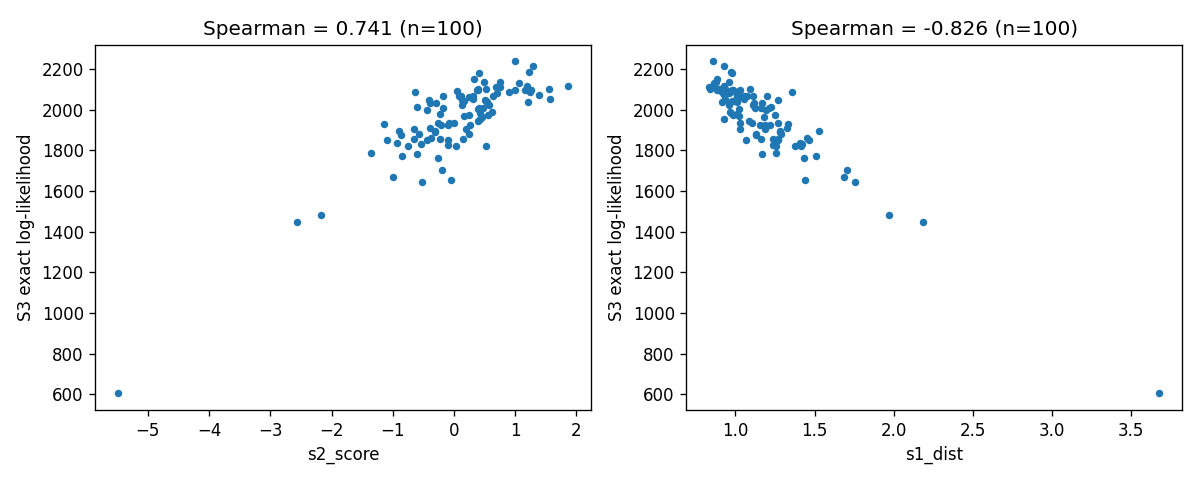
\includegraphics[width=\linewidth]{pool_s3_check.png}

\scriptsize The 100 windows with $S_3$. Left: s2\_score vs log-likelihood. Right: s1\_dist vs log-likelihood (lower distance = more support, so the relation is negative).
\end{column}
\end{columns}
\end{frame}

\begin{frame}{Discriminant validity: support is not quality}
\centering
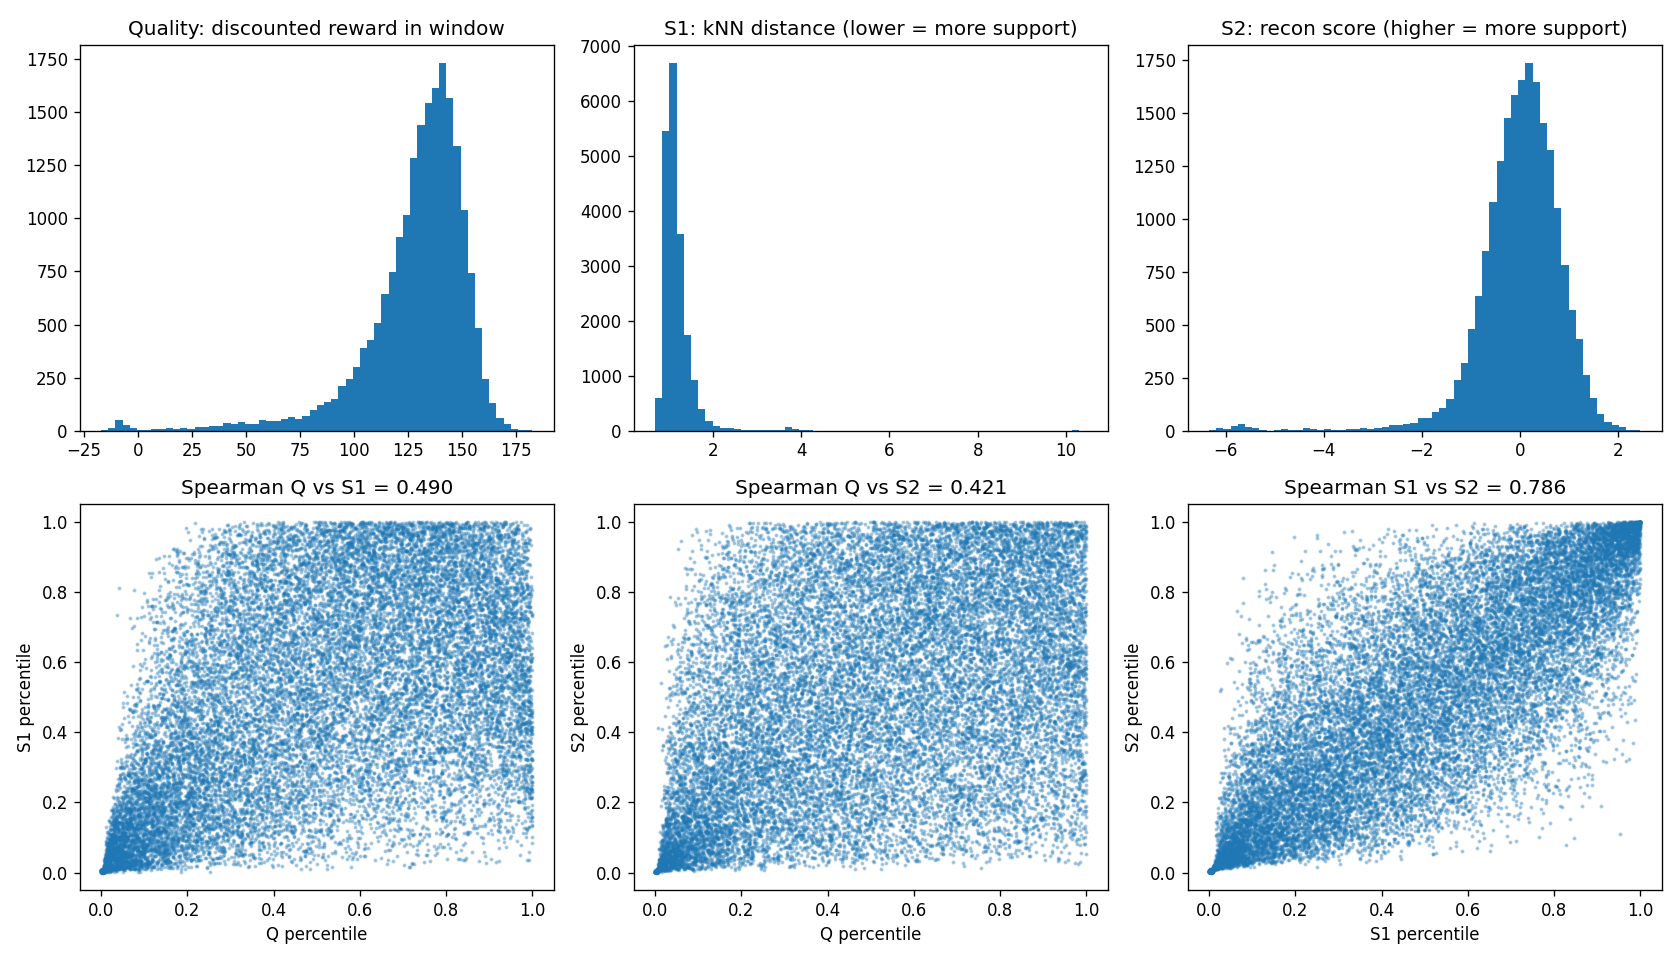
\includegraphics[width=0.8\linewidth]{pool_overview.png}

\raggedright\small 20{,}000 windows. Spearman with quality: $0.49$ ($S_1$), $0.42$ ($S_2$). Related (unusual windows earn less) but far from identical, so they can be studied as two factors.
\end{frame}

\begin{frame}{Predictive validity: support predicts which edits break physics}
400 windows ($5\times5$ grid of quality and support) edited at 7 strengths and replayed in MuJoCo. \textbf{Physics error} = distance between the generated next state and the simulator's next state, in dataset-std units.
\vspace{0.5em}

\centering
\begin{tabular}{lrrrrrrr}
\toprule
$\mu$ & 0.1 & 0.2 & 0.3 & 0.35 & 0.4 & 0.45 & 0.5\\
\midrule
$S_2$ vs physics error & $-0.29$ & $-0.36$ & $-0.34$ & $-0.28$ & $-0.24$ & $-0.18$ & $-0.13$\\
$S_1$ vs physics error & $-0.25$ & $-0.34$ & $-0.32$ & $-0.26$ & $-0.28$ & $-0.25$ & $-0.15$\\
$Q$ vs physics error & $+0.07$ & $+0.01$ & $+0.01$ & $+0.09$ & $+0.04$ & $-0.14$ & $-0.07$\\
\bottomrule
\end{tabular}
\vspace{0.5em}

\raggedright Both support metrics predict which edits break physics, at every editing strength. Quality does not.
\end{frame}

\begin{frame}{Three example windows}
\centering\small
\begin{tabular}{@{}lrrrrrrrrr@{}}
\toprule
 & ep. & start & $q$ & s1\_dist & $e(0.16)$ & $e(0.5)$ & $e(2.4)$ & $S_1$ & $S_2$\\
\midrule
lowest $S_2$ & 593 & 769 & $-8.2$ & 3.82 & 0.0107 & 0.0716 & 0.518 & 0.004 & 0.000\\
median $S_2$ & 738 & 546 & 138.9 & 0.97 & 0.0049 & 0.0213 & 0.135 & 0.80 & 0.50\\
highest $S_2$ & 354 & 552 & 138.3 & 0.77 & 0.0032 & 0.0145 & 0.100 & 0.999 & 1.00\\
\bottomrule
\end{tabular}
\vspace{0.8em}

\raggedright
\begin{itemize}
\item The least supported window earns almost no reward: an unusual moment in which the cheetah barely moves forward.
\item Its nearest other-run neighbours are $\approx4\times$ farther away, and the model's reconstruction errors are 2--5$\times$ larger.
\item $S_1$ and $S_2$ agree on all three windows.
\end{itemize}
\end{frame}

% =====================================================================
\section{Summary}
\begin{frame}{Summary of the three support metrics}
\small
\begin{tabularx}{\linewidth}{@{}lYYY@{}}
\toprule
 & $S_1$ nearest-neighbour & $S_2$ reconstruction & $S_3$ exact log-likelihood\\
\midrule
measures & density of the \textbf{data} around each step & how well the \textbf{model} undoes noise & the \textbf{model's} density of the window\\
looks at & single transitions & whole window & whole window\\
needs the model & no & yes & yes\\
cost (20k windows) & seconds (GPU) & $\approx3$ s (GPU) & 100 windows only\\
strength & direct, model-free & matches what editing uses & exact for the model\\
weakness & ignores step order; arbitrary $k$ & model-dependent; heuristic weights & slow, noisy, model-dependent\\
role & robustness check & \textbf{primary metric} & validation of $S_2$\\
\bottomrule
\end{tabularx}
\end{frame}

\begin{frame}{Conclusions}
\begin{itemize}
\item \textbf{Quality} $Q$ is the discounted reward inside the window: exact.
\item \textbf{Local support} has no ground truth. Three metrics on different assumptions
\begin{itemize}
\item rank windows similarly ($\rho=0.74$--$0.83$),
\item are distinct from quality ($\rho=0.42$--$0.49$),
\item predict the physical validity of edits, while quality does not.
\end{itemize}
\item $S_3$ is a \textbf{reference for $S_2$, not a gold standard}: exact only for the model, noisy per window, 100 windows.
\item Correct claim: ``consistent with each other and predictive of edit validity'', \textbf{not} ``validated against ground truth''.
\end{itemize}
\vspace{0.5em}
\begin{block}{How a true ground-truth test could be built (not done)}
Control support instead of estimating it: remove most data from one region of state space, retrain, and check that $S_1$, $S_2$, $S_3$ fall in that region and only there.
\end{block}
\end{frame}

\begin{frame}{References}
\footnotesize
\begin{itemize}
\item J.\ Lee, S.\ Yun, T.\ Yun, J.\ Park. GTA: Generative Trajectory Augmentation with Guidance for Offline Reinforcement Learning. NeurIPS 2024.
\item T.\ Karras, M.\ Aittala, T.\ Aila, S.\ Laine. Elucidating the Design Space of Diffusion-Based Generative Models. NeurIPS 2022.
\item Y.\ Song, J.\ Sohl-Dickstein, D.\ Kingma, A.\ Kumar, S.\ Ermon, B.\ Poole. Score-Based Generative Modeling through Stochastic Differential Equations. ICLR 2021.
\item Y.\ Song, C.\ Durkan, I.\ Murray, S.\ Ermon. Maximum Likelihood Training of Score-Based Diffusion Models. NeurIPS 2021.
\item D.\ Kingma, T.\ Salimans, B.\ Poole, J.\ Ho. Variational Diffusion Models. NeurIPS 2021.
\item M.\ Hutchinson. A Stochastic Estimator of the Trace of the Influence Matrix for Laplacian Smoothing Splines. Comm.\ Statistics, 1989.
\item J.\ Fu, A.\ Kumar, O.\ Nachum, G.\ Tucker, S.\ Levine. D4RL: Datasets for Deep Data-Driven Reinforcement Learning. 2020.
\end{itemize}
\vspace{0.5em}
\small Code: \texttt{src/h2/quality.py}, \texttt{src/h2/support.py} (\texttt{knn\_distance}, \texttt{recon\_error}, \texttt{log\_likelihood}); run \texttt{python scripts/h2\_run.py pool}.
\end{frame}

\end{document}
